\documentclass[10pt]{beamer}
\usetheme[
%%% option passed to the outer theme
%    progressstyle=fixedCircCnt,   % fixedCircCnt, movingCircCnt (moving is deault)
  ]{Feather}
  
% If you want to change the colors of the various elements in the theme, edit and uncomment the following lines

% Change the bar colors:
%\setbeamercolor{Feather}{fg=red!20,bg=red}

% Change the color of the structural elements:
%\setbeamercolor{structure}{fg=red}

% Change the frame title text color:
%\setbeamercolor{frametitle}{fg=blue}

% Change the normal text color background:
%\setbeamercolor{normal text}{fg=black,bg=gray!10}

%-------------------------------------------------------
% INCLUDE PACKAGES
%-------------------------------------------------------

\usepackage[utf8]{inputenc}
\usepackage[english]{babel}
\usepackage[T1]{fontenc}
\usepackage{helvet}


%-------------------------------------------------------
% DEFFINING AND REDEFINING COMMANDS
%-------------------------------------------------------

% colored hyperlinks
\newcommand{\chref}[2]{
  \href{#1}{{\usebeamercolor[bg]{Feather}#2}}
}

%-------------------------------------------------------
% INFORMATION IN THE TITLE PAGE
%-------------------------------------------------------

\title[] % [] is optional - is placed on the bottom of the sidebar on every slide
{ % is placed on the title page
      \textbf{Bioinfomatics}
}

\subtitle[Sequence Alignment]
{
      \textbf{Sequence Alignment}
}

\author[MSc. Vicente Machaca Arceda]
{      MSc. Vicente Machaca Arceda \\
      {}
}

\institute[]
{
     % {\large \textbf{UNIVERSIDAD NACIONAL DE SAN AGUSTÍN} \\ 
     % Escuela Profesional de Ciencias de la Computación}
     \textbf{UNIVERSIDAD NACIONAL DE SAN AGUSTÍN} \\ 
     Escuela Profesional de Ciencias de la Computación
   
  %there must be an empty line above this line - otherwise some unwanted space is added between the university and the country (I do not know why;( )
}

\date{\today}

%-------------------------------------------------------
% THE BODY OF THE PRESENTATION
%-------------------------------------------------------

\begin{document}


\AtBeginSection[]
{
    \begin{frame}
        \frametitle{Table of Contents}
        \tableofcontents[currentsection]
    \end{frame}
}


%-------------------------------------------------------
% THE TITLEPAGE
%-------------------------------------------------------

{\1% % this is the name of the PDF file for the background
\begin{frame}[plain,noframenumbering] % the plain option removes the header from the title page, noframenumbering removes the numbering of this frame only
  \titlepage % call the title page information from above
\end{frame}}


{\1% % this is the name of the PDF file for the background


%-------------------------------------------------------
%-------------------------------------------------------
%\begin{frame}{Genomes by numbers}{}
%\centering
%\textbf{GENOMES BY NUMBERS} \\
%MSc. Vicente Machaca Arceda 
%\end{frame}
%-------------------------------------------------------
%-------------------------------------------------------

%-------------------------------------------------------
%-------------------------------------------------------
\begin{frame}{Table of Contents}
\tableofcontents
\end{frame}
%-------------------------------------------------------
%-------------------------------------------------------

%%%%%%%%%%%%%%%%%%%%%%%%%%%%%%%%%%%%%%%%%%%%%%%%%%%%%%%%%%%%%%%%%%%%%%%%%%%%%%%%%%%%%%%%%%%%%%%%%%%%%%%%%%%%%%%%
%%%%%%%%%%%%%%%%%%%%%%%%%%%%%%%%%%%%%%%%%%%%%%%%%%%%%%%%%%%%%%%%%%%%%%%%%%%%%%%%%%%%%%%%%%%%%%%%%%%%%%%%%%%%%%%%
\section{Introduction}
%%%%%%%%%%%%%%%%%%%%%%%%%%%%%%%%%%%%%%%%%%%%%%%%%%%%%%%%%%%%%%%%%%%%%%%%%%%%%%%%%%%%%%%%%%%%%%%%%%%%%%%%%%%%%%%%
%%%%%%%%%%%%%%%%%%%%%%%%%%%%%%%%%%%%%%%%%%%%%%%%%%%%%%%%%%%%%%%%%%%%%%%%%%%%%%%%%%%%%%%%%%%%%%%%%%%%%%%%%%%%%%%%

%%%%%%%%%%%%%%%%%%%%%%%%%%%%%%%%%%%%%%%%%%%%%%%%%%%%%%%%%%%%%%%%%%%%%%%%%%%%%%%%%%%%%%%%%%%%%%%%%%%%%%%%%%%%%%%%
%%%%%%%%%%%%%%%%%%%%%%%%%%%%%%%%%%%%%%%%%%%%%%%%%%%%%%%%%%%%%%%%%%%%%%%%%%%%%%%%%%%%%%%%%%%%%%%%%%%%%%%%%%%%%%%%
\subsection{Objectives}
%%%%%%%%%%%%%%%%%%%%%%%%%%%%%%%%%%%%%%%%%%%%%%%%%%%%%%%%%%%%%%%%%%%%%%%%%%%%%%%%%%%%%%%%%%%%%%%%%%%%%%%%%%%%%%%%
%%%%%%%%%%%%%%%%%%%%%%%%%%%%%%%%%%%%%%%%%%%%%%%%%%%%%%%%%%%%%%%%%%%%%%%%%%%%%%%%%%%%%%%%%%%%%%%%%%%%%%%%%%%%%%%%

%-------------------------------------------------------
%-------------------------------------------------------
\begin{frame}{Introduction}{Objectives}
\begin{itemize}
    \item<1-> Understand the importance of sequence alignment in Bioinformatics. 
    \item<2-> Implement the most relevant sequence alignments algorithms.
  \end{itemize}
\end{frame}
%-------------------------------------------------------
%-------------------------------------------------------

%%%%%%%%%%%%%%%%%%%%%%%%%%%%%%%%%%%%%%%%%%%%%%%%%%%%%%%%%%%%%%%%%%%%%%%%%%%%%%%%%%%%%%%%%%%%%%%%%%%%%%%%%%%%%%%%
%%%%%%%%%%%%%%%%%%%%%%%%%%%%%%%%%%%%%%%%%%%%%%%%%%%%%%%%%%%%%%%%%%%%%%%%%%%%%%%%%%%%%%%%%%%%%%%%%%%%%%%%%%%%%%%%
\subsection{Motivation}
%%%%%%%%%%%%%%%%%%%%%%%%%%%%%%%%%%%%%%%%%%%%%%%%%%%%%%%%%%%%%%%%%%%%%%%%%%%%%%%%%%%%%%%%%%%%%%%%%%%%%%%%%%%%%%%%
%%%%%%%%%%%%%%%%%%%%%%%%%%%%%%%%%%%%%%%%%%%%%%%%%%%%%%%%%%%%%%%%%%%%%%%%%%%%%%%%%%%%%%%%%%%%%%%%%%%%%%%%%%%%%%%%

%-------------------------------------------------------
%-------------------------------------------------------
\begin{frame}{Introduction}{Motivation}
\begin{figure}[]
 \centering
    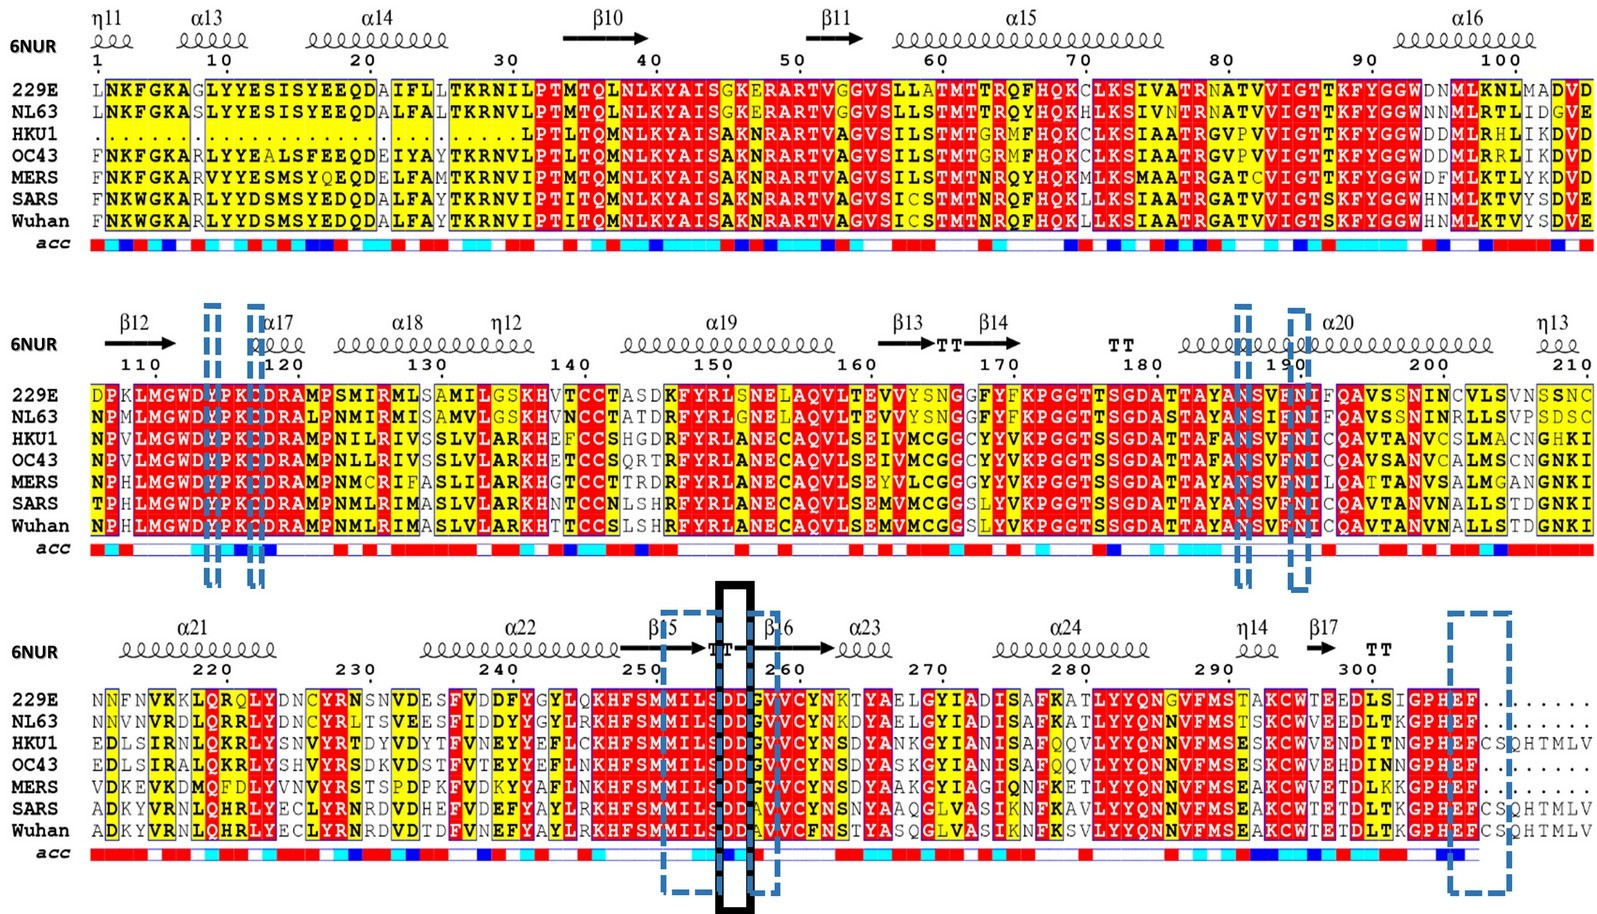
\includegraphics[width=\textwidth,height=0.6\textheight,keepaspectratio]{img/alignment/seq.jpg}
    \label{img:mot2}
    \caption{The SARS HCoV RdRp is the closest strain to the COVID-19, this in-
formation is important for drug designers \cite{elfiky2020anti}.}
\end{figure}
\end{frame}
%-------------------------------------------------------
%-------------------------------------------------------

%-------------------------------------------------------
%-------------------------------------------------------
\begin{frame}{Introduction}{Motivation}
\begin{figure}[]
 \centering
    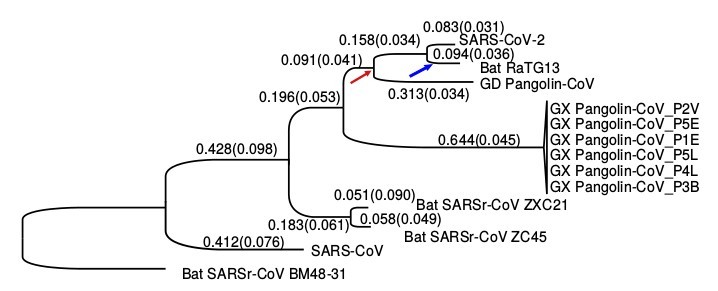
\includegraphics[width=\textwidth,height=0.7\textheight,keepaspectratio]{img/alignment/phylocovid.jpg}
    \label{img:mot2}
    \caption{The phylogenetic tree of SARS-CoV-2 (COVID-19) and the related Coronaviruses  \cite{tang2020origin}.}
\end{figure}
\end{frame}
%-------------------------------------------------------
%-------------------------------------------------------

%%%%%%%%%%%%%%%%%%%%%%%%%%%%%%%%%%%%%%%%%%%%%%%%%%%%%%%%%%%%%%%%%%%%%%%%%%%%%%%%%%%%%%%%%%%%%%%%%%%%%%%%%%%%%%%%
%%%%%%%%%%%%%%%%%%%%%%%%%%%%%%%%%%%%%%%%%%%%%%%%%%%%%%%%%%%%%%%%%%%%%%%%%%%%%%%%%%%%%%%%%%%%%%%%%%%%%%%%%%%%%%%%
\subsection{Previous concepts}
%%%%%%%%%%%%%%%%%%%%%%%%%%%%%%%%%%%%%%%%%%%%%%%%%%%%%%%%%%%%%%%%%%%%%%%%%%%%%%%%%%%%%%%%%%%%%%%%%%%%%%%%%%%%%%%%
%%%%%%%%%%%%%%%%%%%%%%%%%%%%%%%%%%%%%%%%%%%%%%%%%%%%%%%%%%%%%%%%%%%%%%%%%%%%%%%%%%%%%%%%%%%%%%%%%%%%%%%%%%%%%%%%

%-------------------------------------------------------
%-------------------------------------------------------
\begin{frame}{Previous concepts}{Genomic variations}
	\begin{block}{Mutations}
		Many sources of mutation exist that can alter the genome of a cell during its life span, or during replication. Various mutations can affect anything from single base pairs (point mutations), to large genomic regions containing multiple genes.
	\end{block}
\end{frame}
%-------------------------------------------------------
%-------------------------------------------------------



%-------------------------------------------------------
%-------------------------------------------------------
\begin{frame}{Previous concepts}{Mutations types}
	\begin{block}{}
		\begin{itemize}
			\item \textbf{Somatic mutations}, occurs in a single cell and cannot be inherited (cancer).
			\item \textbf{Germline mutations}, occurs in germ cells (sperm and ovum), mutations in these cells can be passed on to offspring.
		\end{itemize}	
	\end{block}
\end{frame}
%-------------------------------------------------------
%-------------------------------------------------------

%-------------------------------------------------------
%-------------------------------------------------------
\begin{frame}{Previous concepts}{Mutations types}
	\begin{block}{}
		\begin{itemize}
			\item \textbf{Point mutations}, are changes to one base in the DNA.
			\item \textbf{Block mutations}, are changes to segments of a chromosome, resulting in large scale changes in the DNA.
		\end{itemize}	
	\end{block}
\end{frame}
%-------------------------------------------------------
%-------------------------------------------------------

%-------------------------------------------------------
%-------------------------------------------------------
\begin{frame}{Previous concepts}{Genomic variations}
	\begin{figure}[]
		\centering
		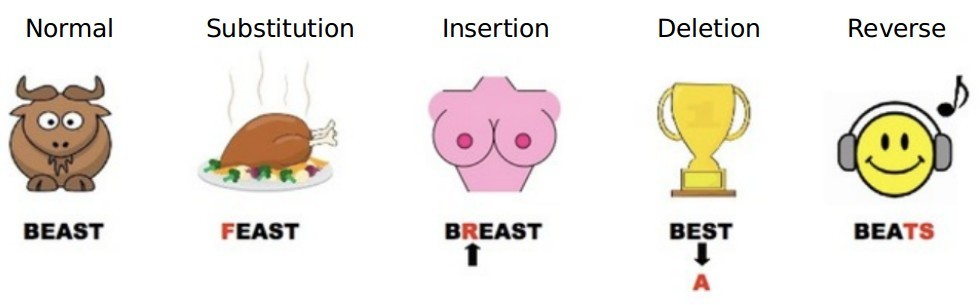
\includegraphics[width=\textwidth,height=0.7\textheight,keepaspectratio]{img/alignment/point_mutations_med.jpg}
		\label{img:alig}
		\caption{Overview of the Different Types of Point Mutations.}
	\end{figure}
\end{frame}
%-------------------------------------------------------
%-------------------------------------------------------

%-------------------------------------------------------
%-------------------------------------------------------
\begin{frame}{Previous concepts}{Genomic variations}
	\begin{figure}[]
		\centering
		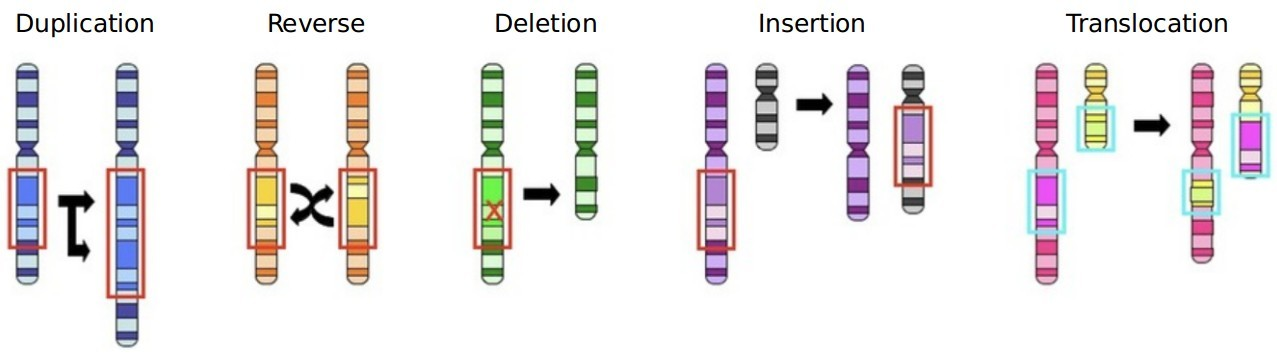
\includegraphics[width=\textwidth,height=0.7\textheight,keepaspectratio]{img/alignment/block_mutations_med.jpg}
		\label{img:alig}
		\caption{Overview of the Different Types of Block Mutations.}
	\end{figure}
\end{frame}
%-------------------------------------------------------
%-------------------------------------------------------

%-------------------------------------------------------
%-------------------------------------------------------
\begin{frame}{Previous concepts}{Genomic variations}
\begin{block}{Inversion}
	A sequence change where, compared to a reference sequence, more than one nucleotide replacing the original sequence are the \textbf{reverse complement} of the original sequence.	
\end{block}
\end{frame}
%-------------------------------------------------------
%-------------------------------------------------------

%-------------------------------------------------------
%-------------------------------------------------------
\begin{frame}{Previous concepts}{Genomic variations}
	\begin{figure}[]
		\centering
		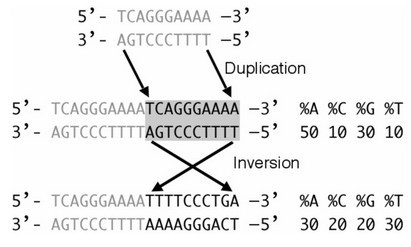
\includegraphics[width=\textwidth,height=0.5\textheight,keepaspectratio]{img/alignment/inv1.jpg}
		\label{img:alig}
		\caption{Inversion example.}
	\end{figure}
\end{frame}
%-------------------------------------------------------
%-------------------------------------------------------


%-------------------------------------------------------
%-------------------------------------------------------
\begin{frame}{Previous concepts}{Genomic variations}
	\begin{figure}[]
		\centering
		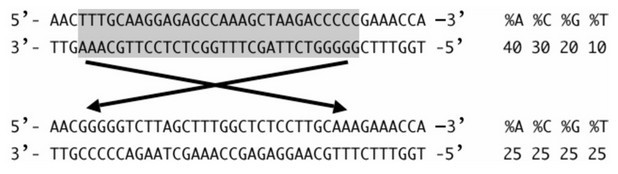
\includegraphics[width=\textwidth,height=0.7\textheight,keepaspectratio]{img/alignment/inv2.jpg}
		\label{img:alig}
		\caption{Inversion example.}
	\end{figure}
\end{frame}
%-------------------------------------------------------
%-------------------------------------------------------

%-------------------------------------------------------
%-------------------------------------------------------
\begin{frame}{Previous concepts}{Genomic variations}
	\begin{block}{Frameshift mutation}
	Also called a framing error or a reading frame shift. It is a genetic mutation (insertions or deletions) of nucleotides that is not divisible by three. 
	\end{block}
	\pause
	\begin{block}{}
	Due to the triplet nature of gene expression by codons, the insertion or deletion can change the reading frame (the grouping of the codons), resulting in a completely different translation from the original.
	\end{block}
\end{frame}
%-------------------------------------------------------
%-------------------------------------------------------

%-------------------------------------------------------
%-------------------------------------------------------
\begin{frame}{Previous concepts}{Genomic variations}
	\begin{figure}[]
		\centering
		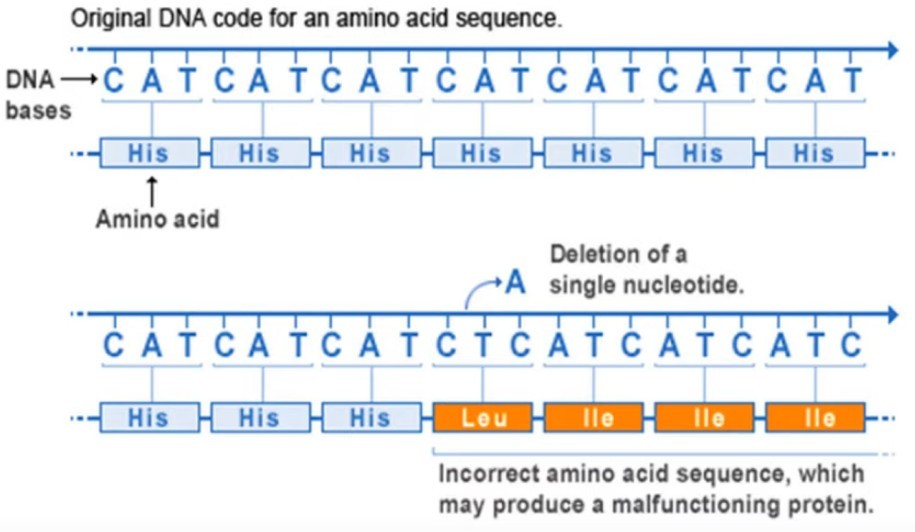
\includegraphics[width=\textwidth,height=0.6\textheight,keepaspectratio]{img/alignment/mut.jpg}
		\label{img:alig}
		\caption{A frameshift mutation cause an incorrect amino acid sequence, which may produce a malfunctioning protein.}
	\end{figure}
\end{frame}
%-------------------------------------------------------
%-------------------------------------------------------

%-------------------------------------------------------
%-------------------------------------------------------
\begin{frame}{Previous concepts}{Genomic variations}
	\begin{block}{}
		Frameshift mutations are apparent in severe genetic diseases such as Tay–Sachs disease (destruction of nerve cells). Also, they increase susceptibility to certain cancers \cite{zimmerman1997inherited}.
	\end{block}
	
\end{frame}
%-------------------------------------------------------
%-------------------------------------------------------

%%%%%%%%%%%%%%%%%%%%%%%%%%%%%%%%%%%%%%%%%%%%%%%%%%%%%%%%%%%%%%%%%%%%%%%%%%%%%%%%%%%%%%%%%%%%%%%%%%%%%%%%%%%%%%%%
%%%%%%%%%%%%%%%%%%%%%%%%%%%%%%%%%%%%%%%%%%%%%%%%%%%%%%%%%%%%%%%%%%%%%%%%%%%%%%%%%%%%%%%%%%%%%%%%%%%%%%%%%%%%%%%%
\section{Sequence alignment}
%%%%%%%%%%%%%%%%%%%%%%%%%%%%%%%%%%%%%%%%%%%%%%%%%%%%%%%%%%%%%%%%%%%%%%%%%%%%%%%%%%%%%%%%%%%%%%%%%%%%%%%%%%%%%%%%
%%%%%%%%%%%%%%%%%%%%%%%%%%%%%%%%%%%%%%%%%%%%%%%%%%%%%%%%%%%%%%%%%%%%%%%%%%%%%%%%%%%%%%%%%%%%%%%%%%%%%%%%%%%%%%%%

%%%%%%%%%%%%%%%%%%%%%%%%%%%%%%%%%%%%%%%%%%%%%%%%%%%%%%%%%%%%%%%%%%%%%%%%%%%%%%%%%%%%%%%%%%%%%%%%%%%%%%%%%%%%%%%%
%%%%%%%%%%%%%%%%%%%%%%%%%%%%%%%%%%%%%%%%%%%%%%%%%%%%%%%%%%%%%%%%%%%%%%%%%%%%%%%%%%%%%%%%%%%%%%%%%%%%%%%%%%%%%%%%
\subsection{Definition}
%%%%%%%%%%%%%%%%%%%%%%%%%%%%%%%%%%%%%%%%%%%%%%%%%%%%%%%%%%%%%%%%%%%%%%%%%%%%%%%%%%%%%%%%%%%%%%%%%%%%%%%%%%%%%%%%
%%%%%%%%%%%%%%%%%%%%%%%%%%%%%%%%%%%%%%%%%%%%%%%%%%%%%%%%%%%%%%%%%%%%%%%%%%%%%%%%%%%%%%%%%%%%%%%%%%%%%%%%%%%%%%%%

%-------------------------------------------------------
%-------------------------------------------------------
\begin{frame}{Sequence alignment}{Definition}

\begin{block}{Pairwise sequence alignment}
\centering
This is the process by which
sequences are compared by searching for common character patterns and establishing residue–residue correspondence among related sequences \cite{xiong2006essential}.
\end{block}

\begin{block}{}
\centering
 It is an important
first step toward structural and functional analysis of newly determined sequences \cite{xiong2006essential}.
\end{block}

\end{frame}
%-------------------------------------------------------
%-------------------------------------------------------


%-------------------------------------------------------
%-------------------------------------------------------
\begin{frame}{Sequence alignment}{Sequence homology versus sequence similarity versus sequence identity}
According to Xiong \cite{xiong2006essential}:
\begin{itemize}
    \item When two sequences are descended from a common evolutionary origin, they have 
homologous relationship or share \textbf{homology}.
    \item Sequence similarity is the \textbf{percentage} of aligned residues that are similar.
    \item Sequence similarity and sequence identity are synonymous for nucleotide sequences but different in a protein sequence. \textbf{Sequence identity} refers to the \textbf{percentage} of matches of the same amino acid residues; \textbf{sequence similarity} refers to the \textbf{percentage} of aligned residues that have similar physicochemical characteristics ( size, charge, and hydrophobicity).

\end{itemize}
\end{frame}
%-------------------------------------------------------
%-------------------------------------------------------


%-------------------------------------------------------
%-------------------------------------------------------
\begin{frame}{Sequence alignment}{Examples}
\begin{columns}
	\begin{column}{0.48\textwidth}
		\begin{figure}[]
			\centering
			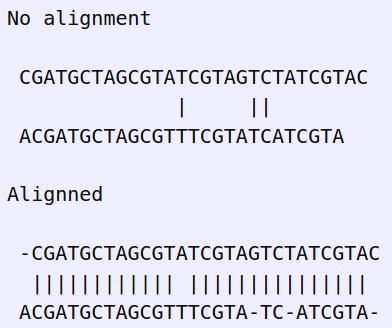
\includegraphics[width=\textwidth,height=0.6\textheight,keepaspectratio]{img/alignment/al1.jpg}
			\label{img:alig}
			\caption{No alignment versus alignment.}
		\end{figure}
	\end{column}
	\begin{column}{0.48\textwidth}
		In the alignment process there could be substitutions, changes of residues and gaps. Gaps could cause by insertions or deletions.
	\end{column}
\end{columns}
\end{frame}
%-------------------------------------------------------
%-------------------------------------------------------

%-------------------------------------------------------
%-------------------------------------------------------
\begin{frame}{Sequence alignment}{Examples}
\begin{columns}
	\begin{column}{0.48\textwidth}
		\begin{figure}[]
			\centering
			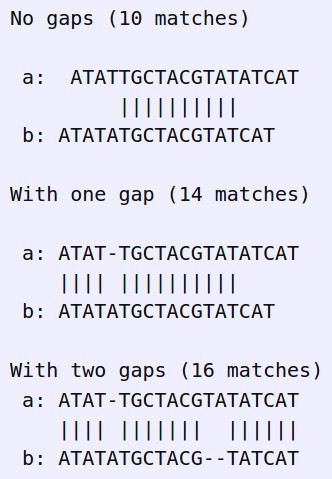
\includegraphics[width=\textwidth,height=0.7\textheight,keepaspectratio]{img/alignment/al2.jpg}
			\label{img:alig}
			\caption{Alignment and gaps.}
		\end{figure}
	\end{column}
	\begin{column}{0.48\textwidth}
		Algorithms should take into account the possibility of introducing gaps. \textbf{Several alignments can be constructed} between two sequences.
	\end{column}
\end{columns}
	
\end{frame}
%-------------------------------------------------------
%-------------------------------------------------------

%-------------------------------------------------------
%-------------------------------------------------------
\begin{frame}{Sequence alignment}{Evaluating the alignments}
To compare alignments we can score them. The main features taken into account are usually: 
\begin{itemize}
	\item Number of matching residues.
	\item Number of missmatches.
	\item Number of gaps.
	\item Length of the gaps.
\end{itemize}
\end{frame}
%-------------------------------------------------------
%-------------------------------------------------------

%-------------------------------------------------------
%-------------------------------------------------------
\begin{frame}{Sequence alignment}{Evaluating the alignments}
	We can devise different scoring schemes. For instances:
	\begin{itemize}
		\item scoring schema 1: match +1, mismatch: 0, gap creation: -1 gap extension: -1
		\item scoring schema 1: match +1, mismatch: -1, gap creation: -1 gap extension: 0
	\end{itemize}
\end{frame}
%-------------------------------------------------------
%-------------------------------------------------------



%-------------------------------------------------------
%-------------------------------------------------------
\begin{frame}{Sequence alignment}{Global Alignment and Local Alignment}

\begin{block}{}
\centering
In \textbf{Global alignment}, two sequences to be aligned are assumed to be generally similar over their entire length. Alignment is carried out from beginning to end \cite{xiong2006essential}.
\end{block}
\begin{block}{}
\centering
\textbf{Local alignment}, does not assume that the two sequences have similarity over the entire length. It only finds local regions with the highest level of similarity \cite{xiong2006essential}.
\end{block}
\end{frame}
%-------------------------------------------------------
%-------------------------------------------------------


%-------------------------------------------------------
%-------------------------------------------------------
\begin{frame}{Sequence alignment}{Global Alignment and Local Alignment}
\begin{figure}[]
 \centering
    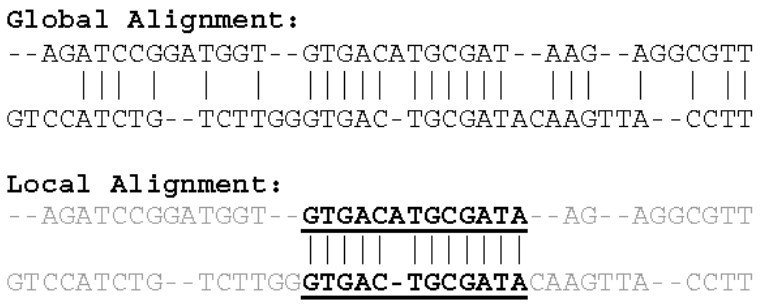
\includegraphics[width=\textwidth,height=0.7\textheight,keepaspectratio]{img/alignment/alig.jpg}
    \label{img:alig}
    \caption{Global Alignment and Local Alignment.}
\end{figure}
\end{frame}
%-------------------------------------------------------
%-------------------------------------------------------

%-------------------------------------------------------
%-------------------------------------------------------
\begin{frame}{Sequence alignment}{Alignment Algorithms}
Global and local, are fundamentally similar and only differ in the optimization strategy used in aligning similar residues, the algorithms can be based on one of the three methods:
\begin{itemize}
    \item The dot matrix method.
    \item The dynamic programming method.
    \item The word method.
\end{itemize}
\end{frame}
%-------------------------------------------------------
%-------------------------------------------------------

%%%%%%%%%%%%%%%%%%%%%%%%%%%%%%%%%%%%%%%%%%%%%%%%%%%%%%%%%%%%%%%%%%%%%%%%%%%%%%%%%%%%%%%%%%%%%%%%%%%%%%%%%%%%%%%%
%%%%%%%%%%%%%%%%%%%%%%%%%%%%%%%%%%%%%%%%%%%%%%%%%%%%%%%%%%%%%%%%%%%%%%%%%%%%%%%%%%%%%%%%%%%%%%%%%%%%%%%%%%%%%%%%
\subsection{Dot matrix}                                 %%%%%%%%%%%%%%%%%%%%%%%%%%%%%%%%%%%%%%%%%%%%%%%%%%%%%%%%
%%%%%%%%%%%%%%%%%%%%%%%%%%%%%%%%%%%%%%%%%%%%%%%%%%%%%%%%%%%%%%%%%%%%%%%%%%%%%%%%%%%%%%%%%%%%%%%%%%%%%%%%%%%%%%%%
%%%%%%%%%%%%%%%%%%%%%%%%%%%%%%%%%%%%%%%%%%%%%%%%%%%%%%%%%%%%%%%%%%%%%%%%%%%%%%%%%%%%%%%%%%%%%%%%%%%%%%%%%%%%%%%%

%-------------------------------------------------------
%-------------------------------------------------------
\begin{frame}{Sequence alignment}{Dot matrix}

\begin{block}{Dot matrix}
\centering
The most basic sequence alignment method is the \textbf{Dot matrix} method, proposed by Gibbs and McIntyre (1970) \cite{gibbs1970diagram}, also known
as the \textbf{Dot plot} method. It is a graphical way of comparing two sequences in a two 
dimensional matrix \cite{xiong2006essential}.
\end{block}

\end{frame}
%-------------------------------------------------------
%-------------------------------------------------------

%-------------------------------------------------------
%-------------------------------------------------------
\begin{frame}{Sequence alignment}{Dot matrix}

\begin{figure}[]
 \centering
    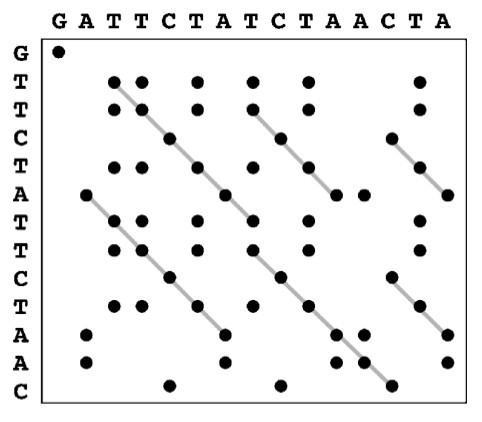
\includegraphics[width=\textwidth,height=0.7\textheight,keepaspectratio]{img/alignment/dot.jpg}
    \label{img:uniprot}
    \caption{Dot matrix example}
\end{figure}
\end{frame}
%-------------------------------------------------------
%-------------------------------------------------------

%-------------------------------------------------------
%-------------------------------------------------------
\begin{frame}{Sequence alignment}{Dot matrix}
	
	\begin{figure}[]
		\centering
		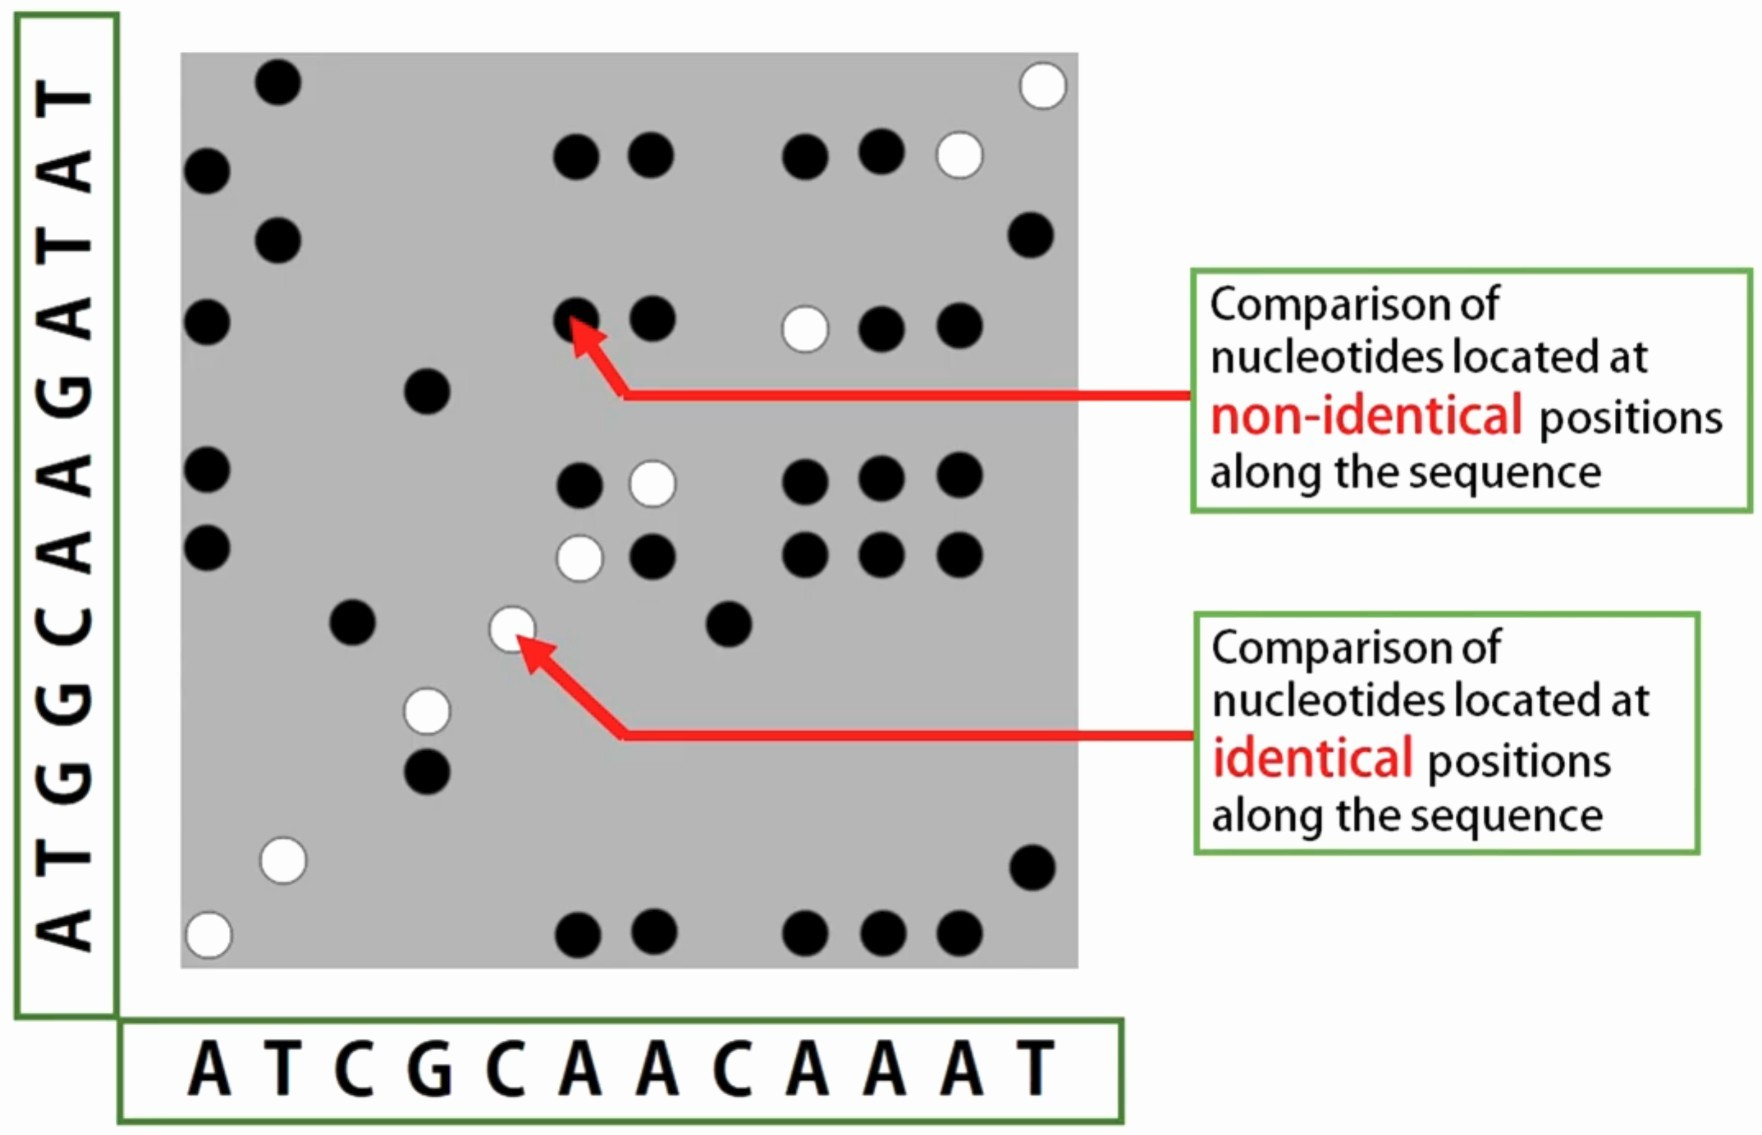
\includegraphics[width=\textwidth,height=0.7\textheight,keepaspectratio]{img/alignment/dot_plot4.jpg}
		\label{img:uniprot}
		\caption{Dot matrix example}
	\end{figure}
\end{frame}
%-------------------------------------------------------
%-------------------------------------------------------


%-------------------------------------------------------
%-------------------------------------------------------
\begin{frame}{Sequence alignment}{Dot matrix}
	\centering
	\textbf{What we could conclude from the Dot plot?}	 
	\begin{figure}[]		
		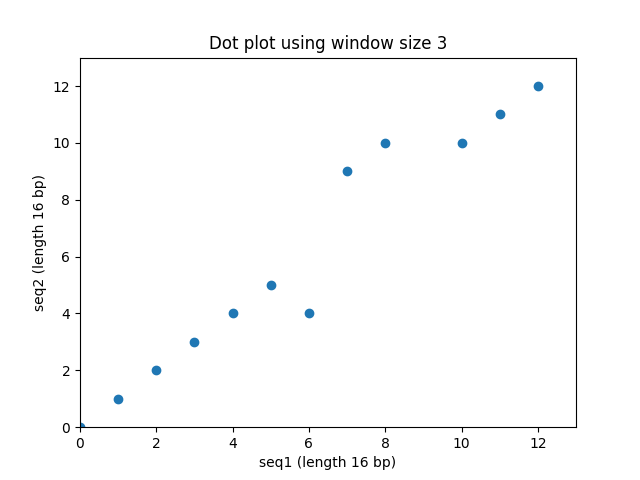
\includegraphics[width=\textwidth,height=0.5\textheight,keepaspectratio]{img/alignment/dot_plot1.png}
		\label{img:uniprot}
		\caption{Dot matrix example. $seq1 = ACCTGAGAGTGTGGCT$ and $seq2 = ACCTGAGACAGTGGCT$}
	\end{figure}
\end{frame}
%-------------------------------------------------------
%-------------------------------------------------------

%-------------------------------------------------------
%-------------------------------------------------------
\begin{frame}{Sequence alignment}{Dot matrix}
	\centering
	\textbf{What we could conclude from the Dot plot?}	 
	\begin{figure}[]		
		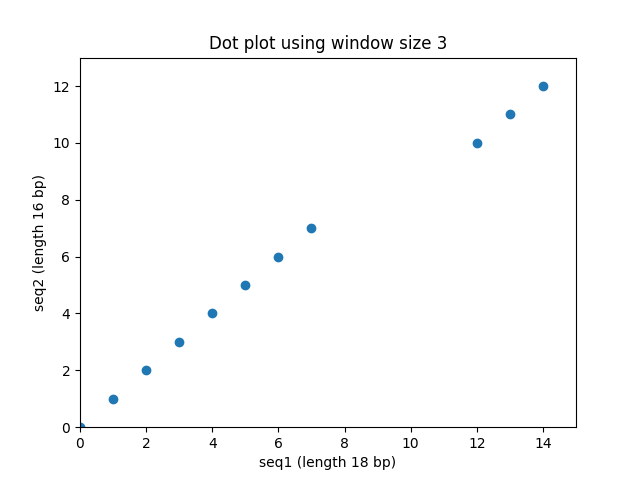
\includegraphics[width=\textwidth,height=0.5\textheight,keepaspectratio]{img/alignment/dot_plot2.png}
		\label{img:uniprot}
		\caption{Dot matrix example. $seq1 = ACCTGAGACATTGTGGCT$ and $seq2 = ACCTGAGACAGTGGCT$}
	\end{figure}
\end{frame}
%-------------------------------------------------------
%-------------------------------------------------------

%-------------------------------------------------------
%-------------------------------------------------------
\begin{frame}{Sequence alignment}{Dot matrix}
	\centering
	\textbf{What we could conclude from the Dot plot?}	 
	\begin{figure}[]		
		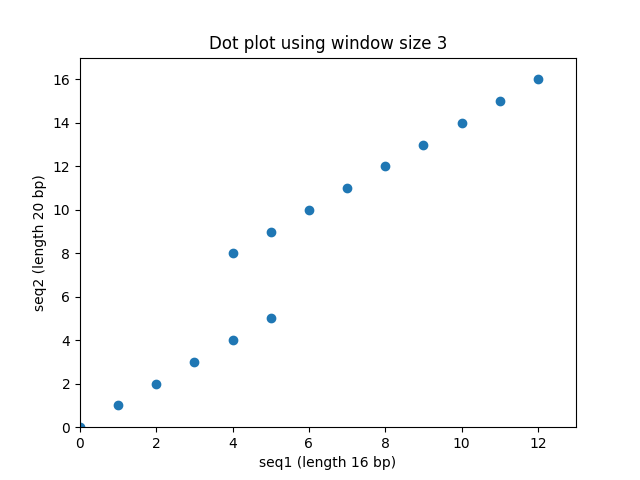
\includegraphics[width=\textwidth,height=0.5\textheight,keepaspectratio]{img/alignment/dot_plot3.png}
		\label{img:uniprot}
		\caption{Dot matrix example. $seq1 = ACCTGATACAGTGGCT$ and $seq2 = ACCTGATAGATACAGTGGCT$}
	\end{figure}
\end{frame}
%-------------------------------------------------------
%-------------------------------------------------------

%-------------------------------------------------------
%-------------------------------------------------------
\begin{frame}{Sequence alignment}{Dot matrix}
	
	\begin{figure}[]
		\centering
		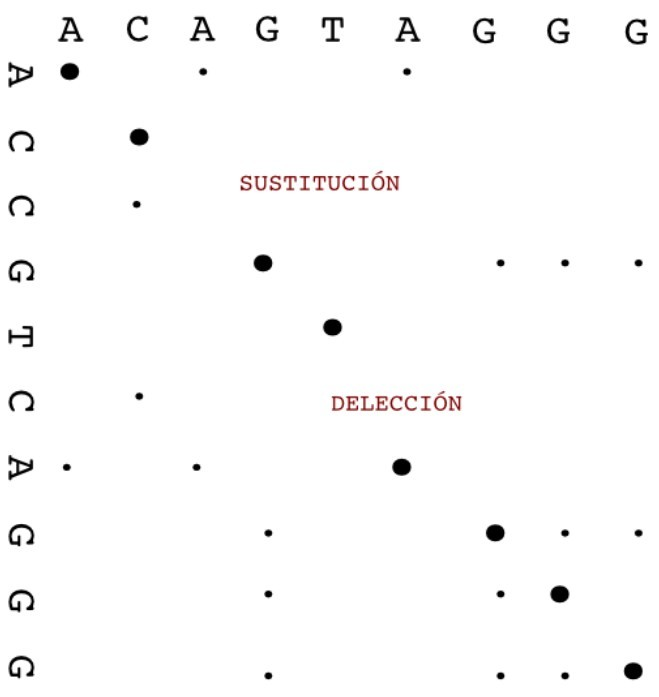
\includegraphics[width=\textwidth,height=0.7\textheight,keepaspectratio]{img/alignment/al3.jpg}
		\label{img:uniprot}
		\caption{Dot matrix example}
	\end{figure}
\end{frame}
%-------------------------------------------------------
%-------------------------------------------------------

%-------------------------------------------------------
%-------------------------------------------------------
\begin{frame}{Sequence alignment}{Dot matrix}
	
	\begin{figure}[]
		\centering
		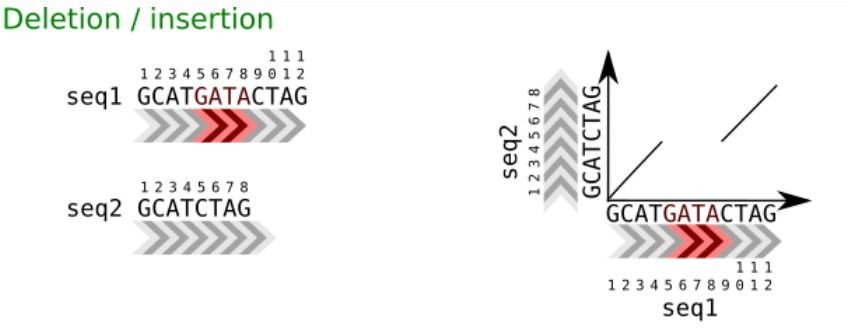
\includegraphics[width=\textwidth,height=0.7\textheight,keepaspectratio]{img/alignment/al4.jpg}
		\label{img:uniprot}
		\caption{Deletion/insertion example in Dot matrix.}
	\end{figure}
\end{frame}
%-------------------------------------------------------
%-------------------------------------------------------

%-------------------------------------------------------
%-------------------------------------------------------
\begin{frame}{Sequence alignment}{Dot matrix}
	
	\begin{figure}[]
		\centering
		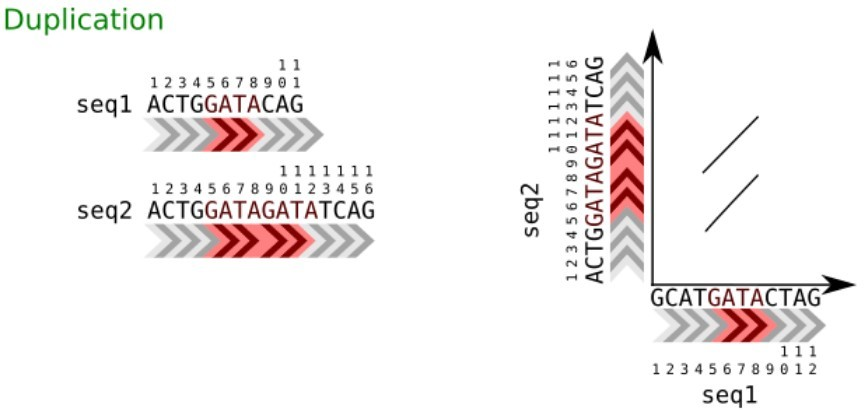
\includegraphics[width=\textwidth,height=0.7\textheight,keepaspectratio]{img/alignment/al5.jpg}
		\label{img:uniprot}
		\caption{Duplication example in Dot matrix.}
	\end{figure}
\end{frame}
%-------------------------------------------------------
%-------------------------------------------------------

%-------------------------------------------------------
%-------------------------------------------------------
%\begin{frame}{Sequence alignment}{Dot matrix}
	
%	\begin{figure}[]
%		\centering
%		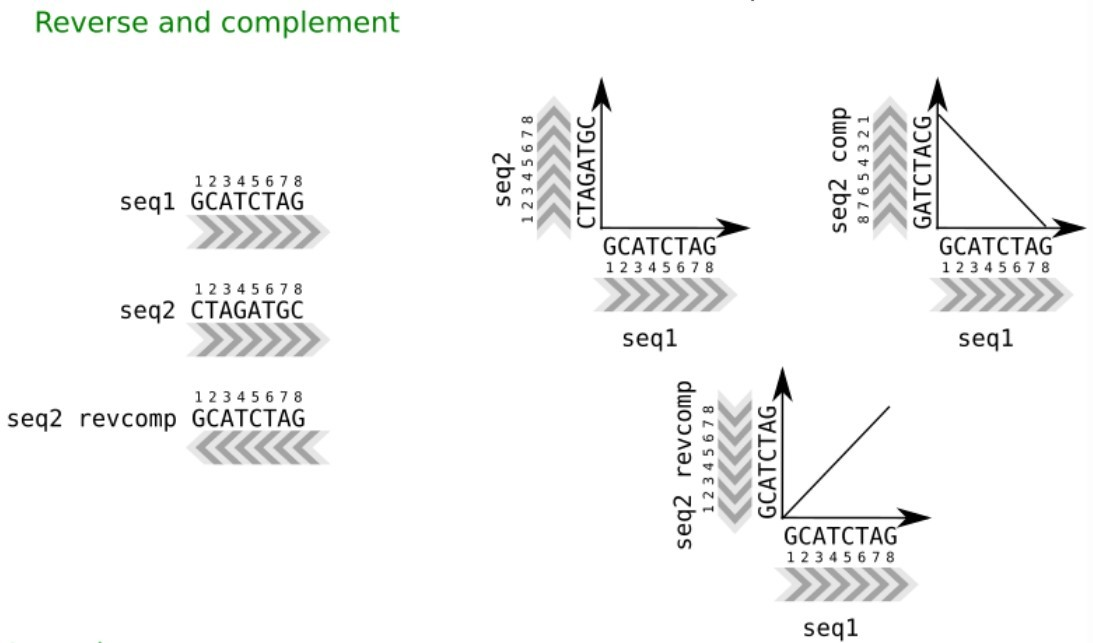
\includegraphics[width=\textwidth,height=0.7\textheight,keepaspectratio]{img/alignment/al6.jpg}
%		\label{img:uniprot}
%		\caption{Reverse and complement example in Dot matrix.}
%	\end{figure}
%\end{frame}
%-------------------------------------------------------
%-------------------------------------------------------

%-------------------------------------------------------
%-------------------------------------------------------
%\begin{frame}{Sequence alignment}{Dot matrix}
	
%	\begin{figure}[]
%		\centering
%		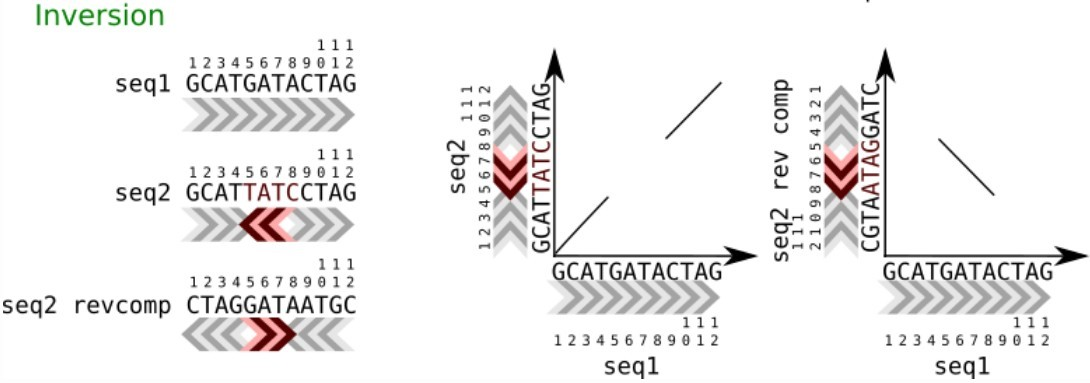
\includegraphics[width=\textwidth,height=0.7\textheight,keepaspectratio]{img/alignment/al7.jpg}
%		\label{img:uniprot}
%		\caption{Inversion (reverse-complement) example in Dot matrix.}
%	\end{figure}
%\end{frame}
%-------------------------------------------------------
%-------------------------------------------------------

%https://bioinf.comav.upv.es/courses/biotech3/theory/sequence_alignment.html

%-------------------------------------------------------
%-------------------------------------------------------
\begin{frame}{Sequence alignment}{Noise in Dot matrix}	
	\begin{figure}[]
		\centering
		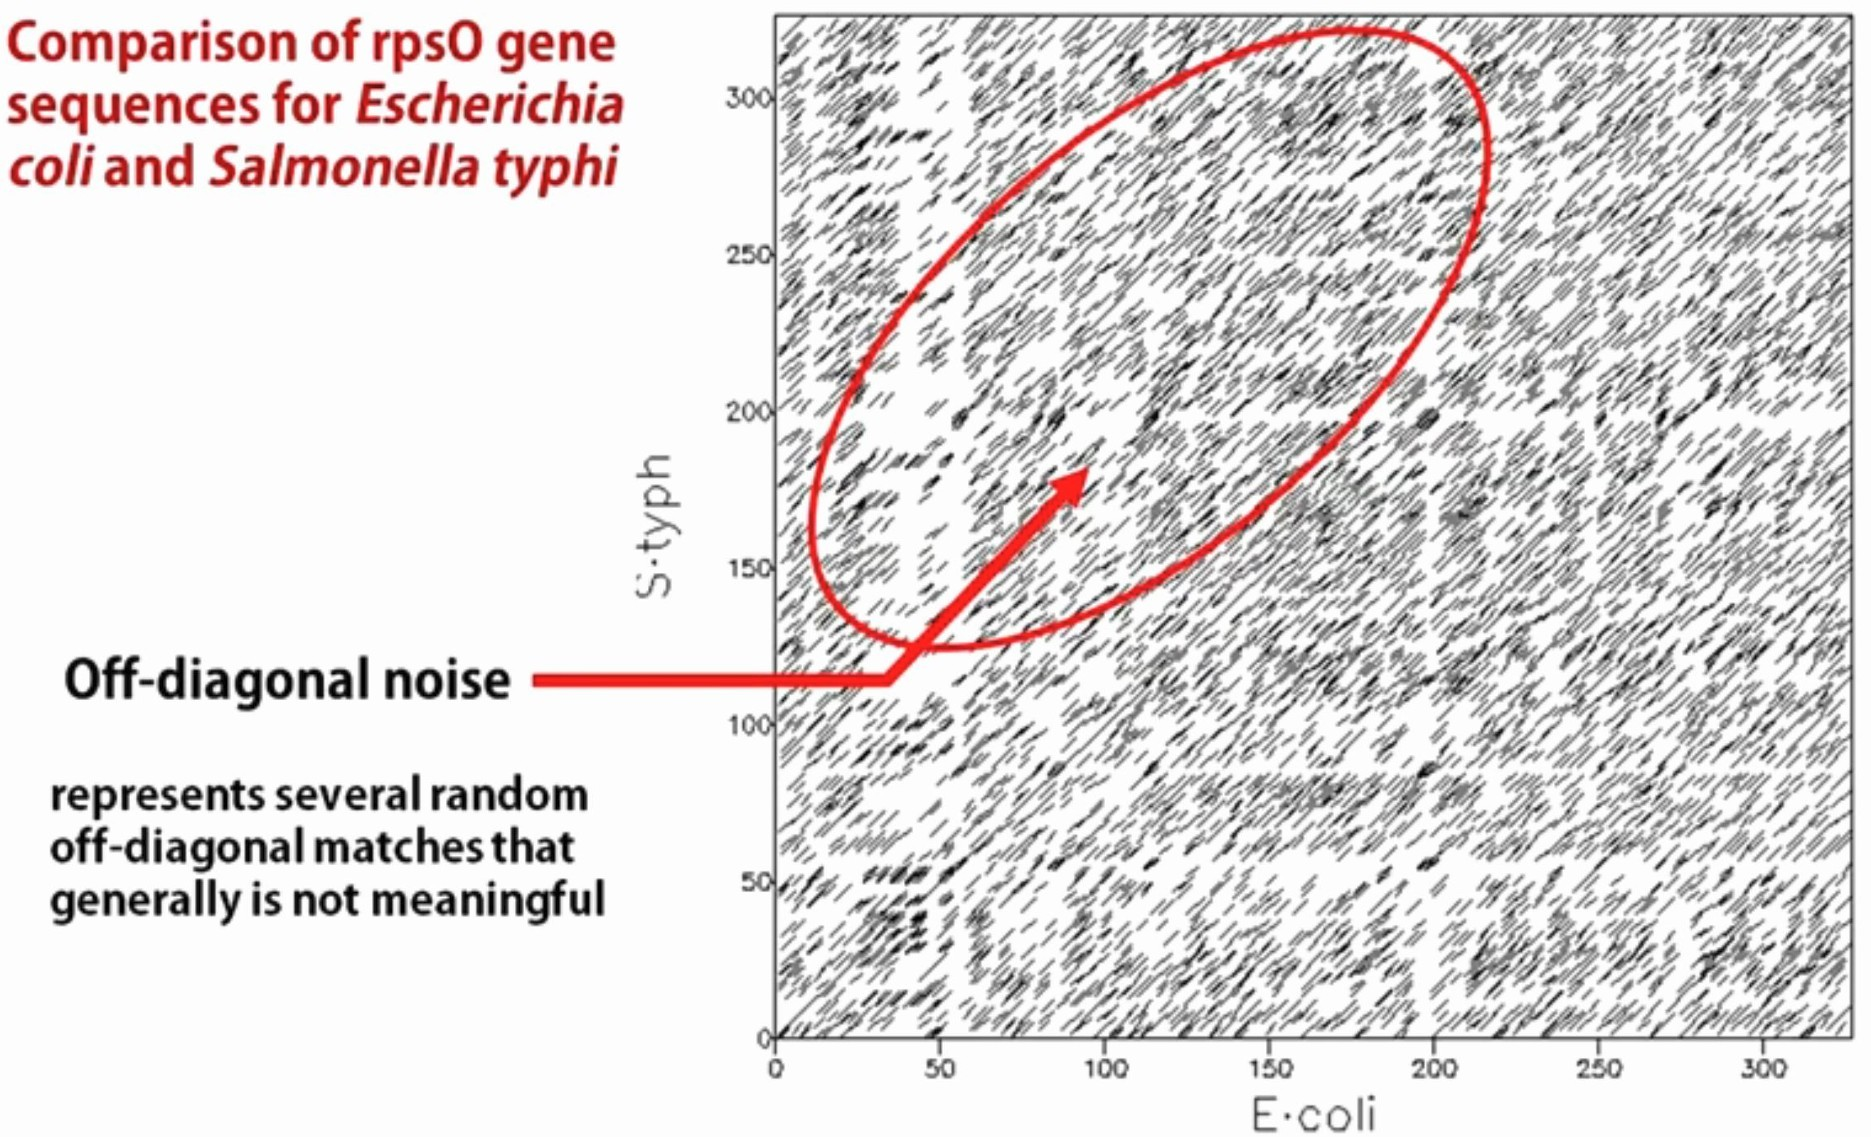
\includegraphics[width=\textwidth,height=0.6\textheight,keepaspectratio]{img/alignment/dot_plot5.jpg}
		\label{img:uniprot}
		\caption{Several off-diagonal matches that generally is not meaningfull.}
	\end{figure}
\end{frame}
%-------------------------------------------------------
%-------------------------------------------------------

%-------------------------------------------------------
%-------------------------------------------------------
\begin{frame}{Sequence alignment}{Dot matrix with window size}	
	\begin{figure}[]
		\centering
		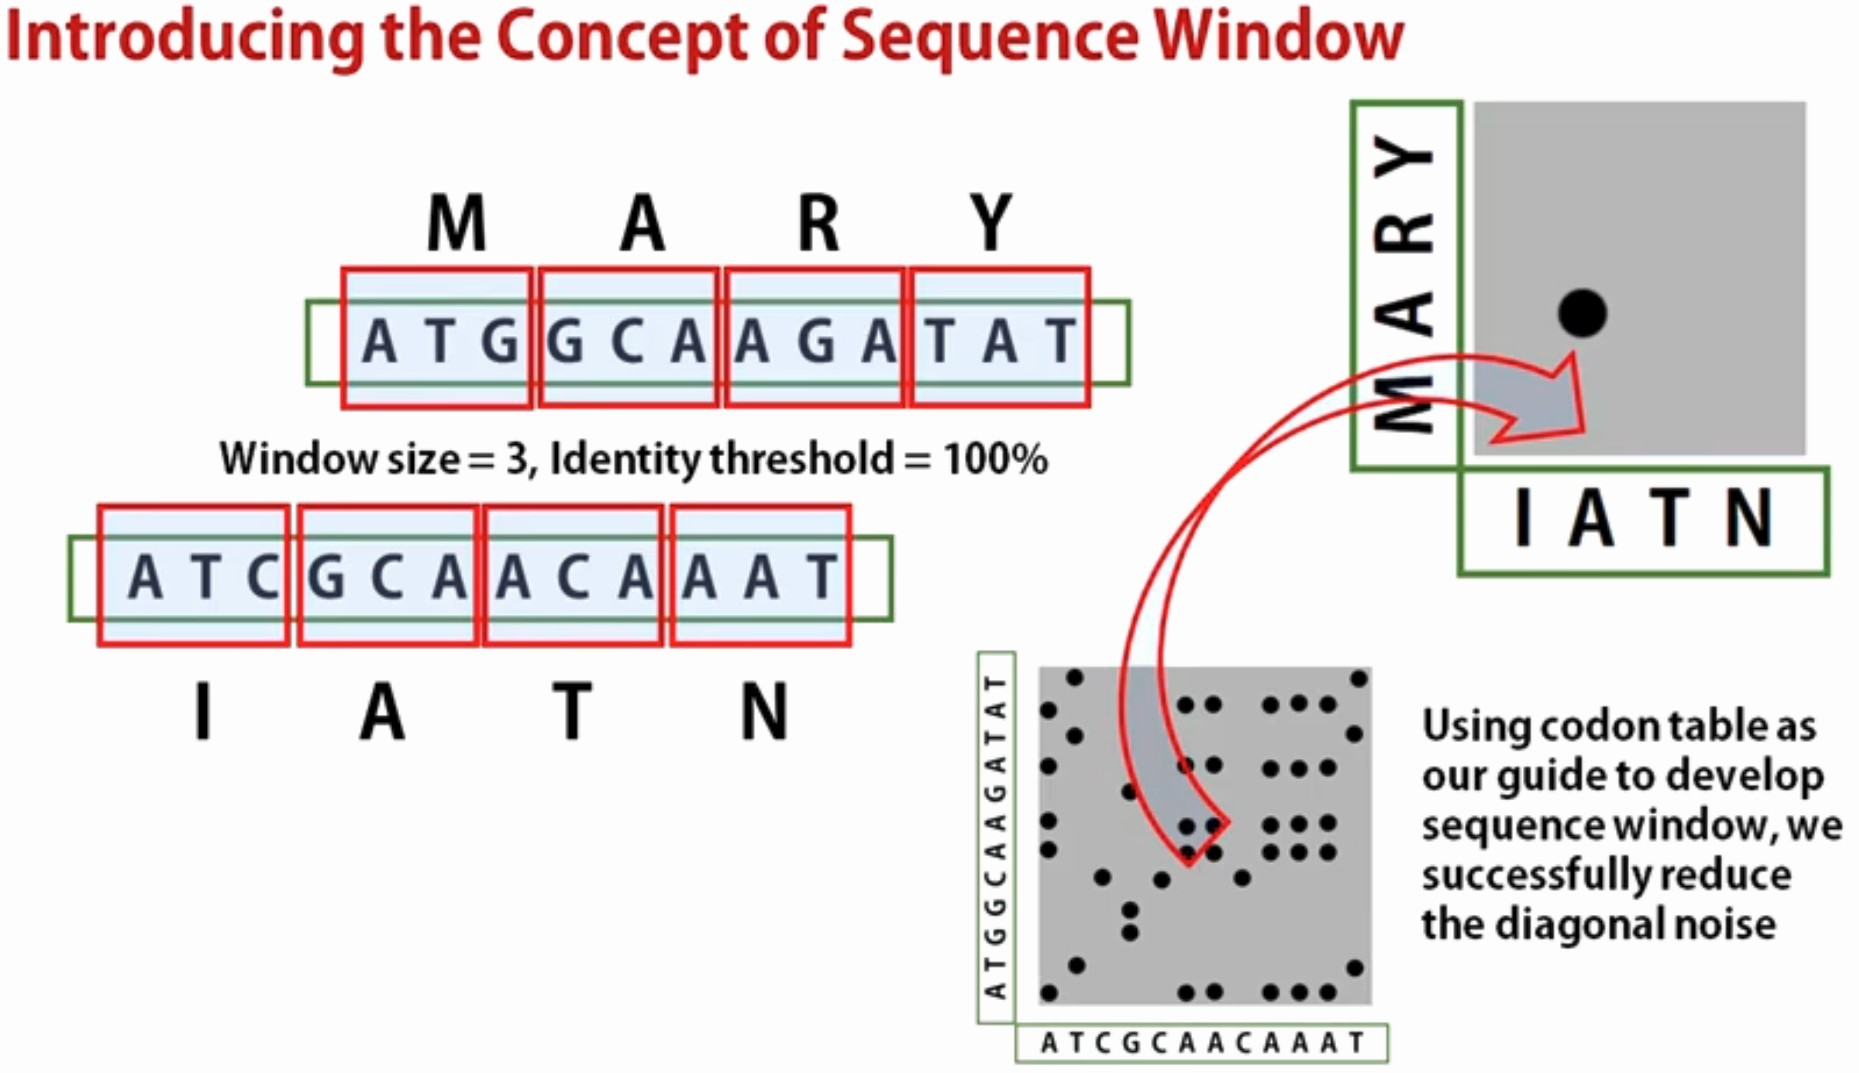
\includegraphics[width=\textwidth,height=0.6\textheight,keepaspectratio]{img/alignment/dot_plot6.jpg}
		\label{img:uniprot}
		\caption{Dot plot with windows successfully reduce the diagonal noise.}
	\end{figure}
\end{frame}
%-------------------------------------------------------
%-------------------------------------------------------

%-------------------------------------------------------
%-------------------------------------------------------
\begin{frame}{Sequence alignment}{Dot matrix with window size}	
	\begin{figure}[]
		\centering
		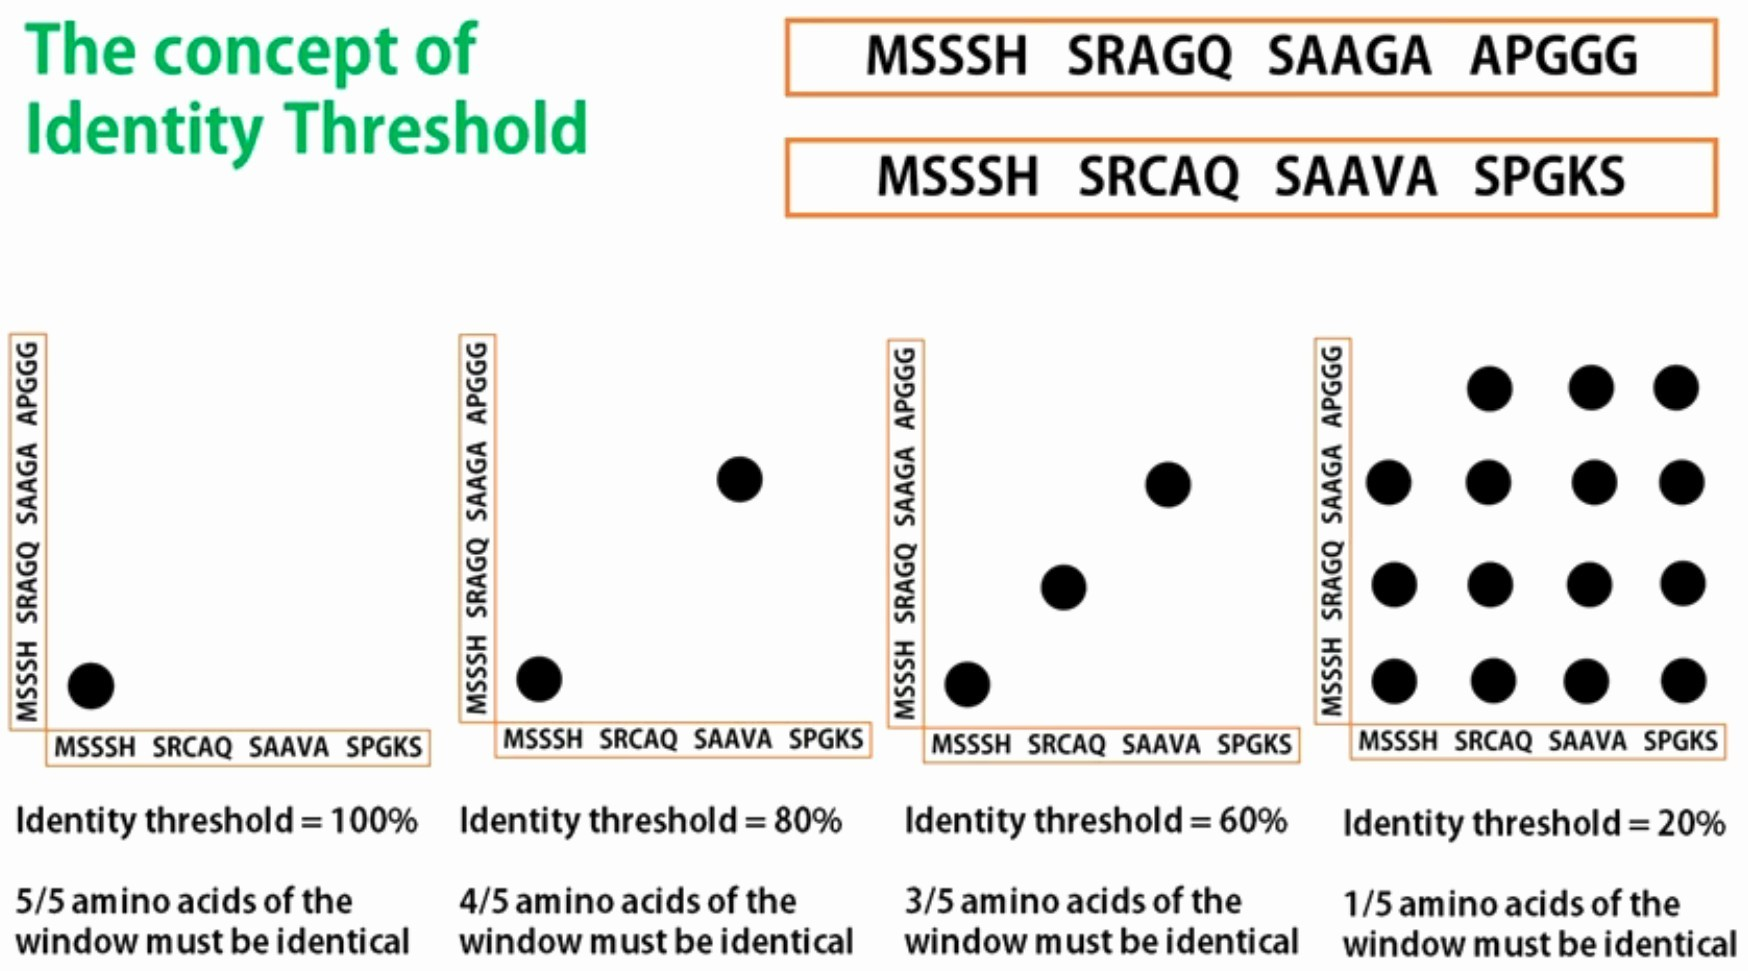
\includegraphics[width=\textwidth,height=0.6\textheight,keepaspectratio]{img/alignment/dot_plot7.jpg}
		\label{img:uniprot}
		\caption{According to identity threshold, different dot plots are obtained.}
	\end{figure}
\end{frame}
%-------------------------------------------------------
%-------------------------------------------------------

%%%%%%%%%%%%%%%%%%%%%%%%%%%%%%%%%%%%%%%%%%%%%%%%%%%%%%%%%%%%%%%%%%%%%%%%%%%%%%%%%%%%%%%%%%%%%%%%%%%%%%%%%%%%%%%%
%%%%%%%%%%%%%%%%%%%%%%%%%%%%%%%%%%%%%%%%%%%%%%%%%%%%%%%%%%%%%%%%%%%%%%%%%%%%%%%%%%%%%%%%%%%%%%%%%%%%%%%%%%%%%%%%
\subsection{Practice}                                 %%%%%%%%%%%%%%%%%%%%%%%%%%%%%%%%%%%%%%%%%%%%%%%%%%%%%%%%
%%%%%%%%%%%%%%%%%%%%%%%%%%%%%%%%%%%%%%%%%%%%%%%%%%%%%%%%%%%%%%%%%%%%%%%%%%%%%%%%%%%%%%%%%%%%%%%%%%%%%%%%%%%%%%%%
%%%%%%%%%%%%%%%%%%%%%%%%%%%%%%%%%%%%%%%%%%%%%%%%%%%%%%%%%%%%%%%%%%%%%%%%%%%%%%%%%%%%%%%%%%%%%%%%%%%%%%%%%%%%%%%%

%-------------------------------------------------------
%-------------------------------------------------------
\begin{frame}{Sequence alignment}{Practice}
Now, we are going to see how Dot matrix is compute using online tools. Follow the next steps:
\begin{itemize}
    \item Download sample genomes.
    \item Visit the online tool.
    \item Interpret the results.
\end{itemize}
\end{frame}
%-------------------------------------------------------
%-------------------------------------------------------

%-------------------------------------------------------
%-------------------------------------------------------
\begin{frame}{Sequence alignment}{Practice}
Visit this website in order to download the genomes: \href{https://www.uniprot.org/}{UniProt} 
\begin{figure}[]
 \centering
    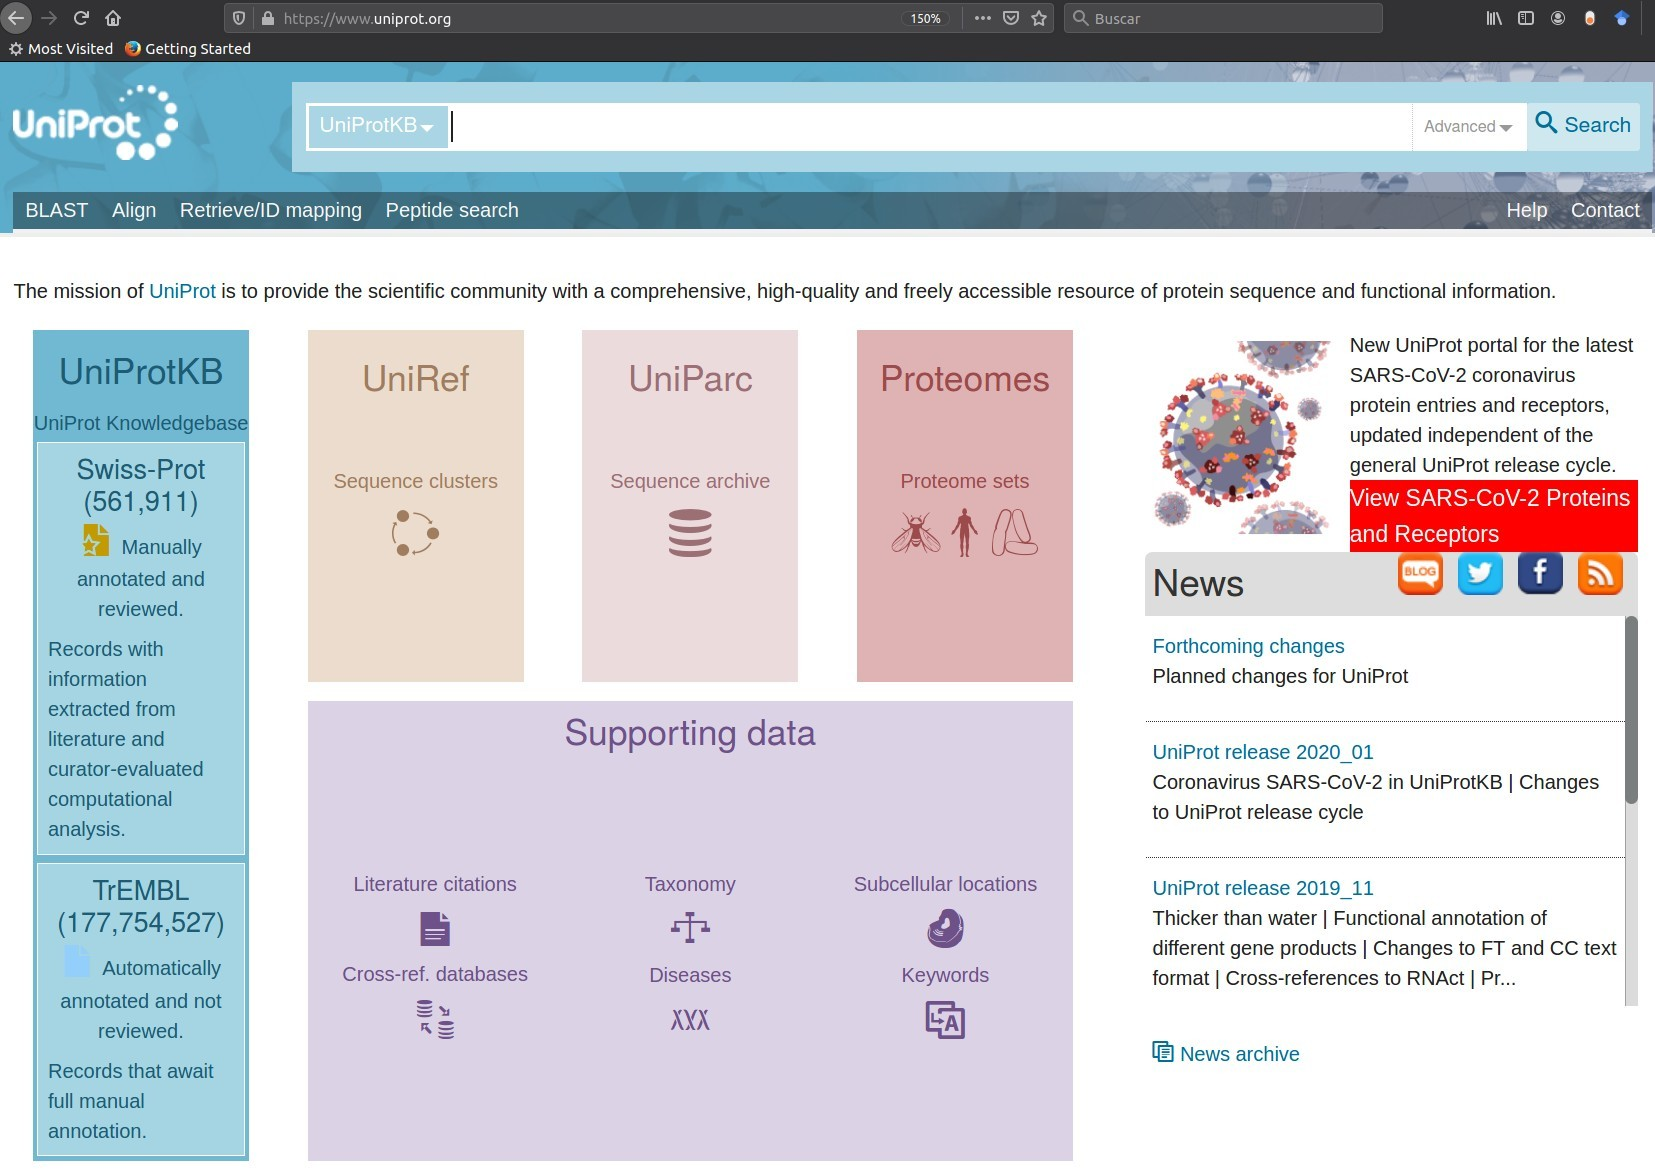
\includegraphics[width=\textwidth,height=0.7\textheight,keepaspectratio]{img/alignment/uniprot.jpg}
    \label{img:uniprot}
    \caption{UniProt: Database of proteins and genomes.}
\end{figure}
\end{frame}
%-------------------------------------------------------
%-------------------------------------------------------

%-------------------------------------------------------
%-------------------------------------------------------
\begin{frame}{Sequence alignment}{Practice}
Search the Filamin-A protein of a human species. 
\begin{figure}[]
 \centering
    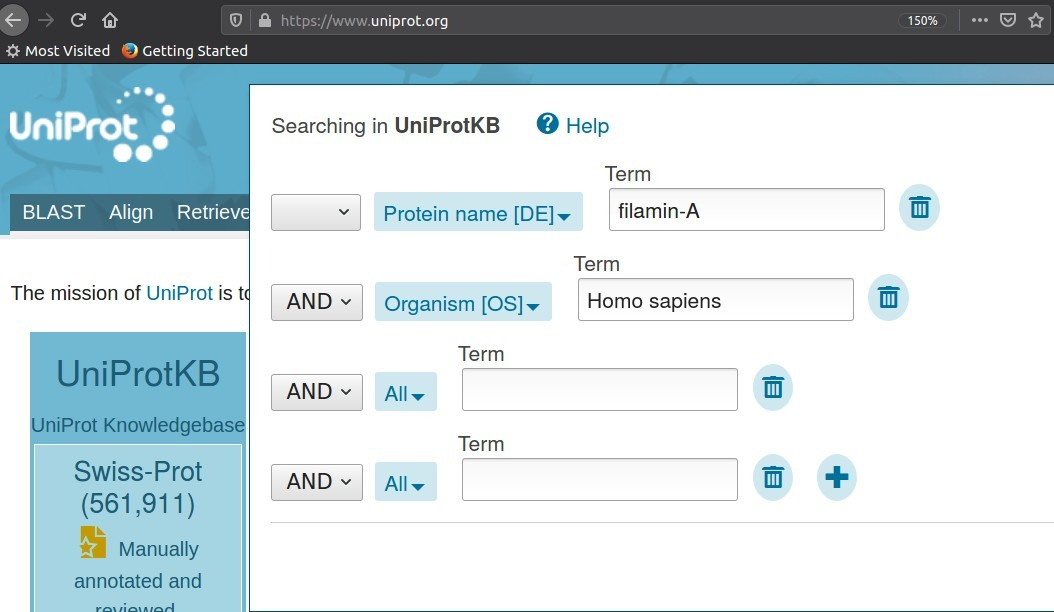
\includegraphics[width=\textwidth,height=0.7\textheight,keepaspectratio]{img/alignment/uniprot2.jpg}
    \label{img:uniprot2}
    \caption{Searching the Filamin-A protein of a human  species}
\end{figure}
\end{frame}
%-------------------------------------------------------
%-------------------------------------------------------

%-------------------------------------------------------
%-------------------------------------------------------
\begin{frame}{Sequence alignment}{Practice}
Select the sequence P21333 (its length is \string ~2.6). 
\begin{figure}[]
 \centering
    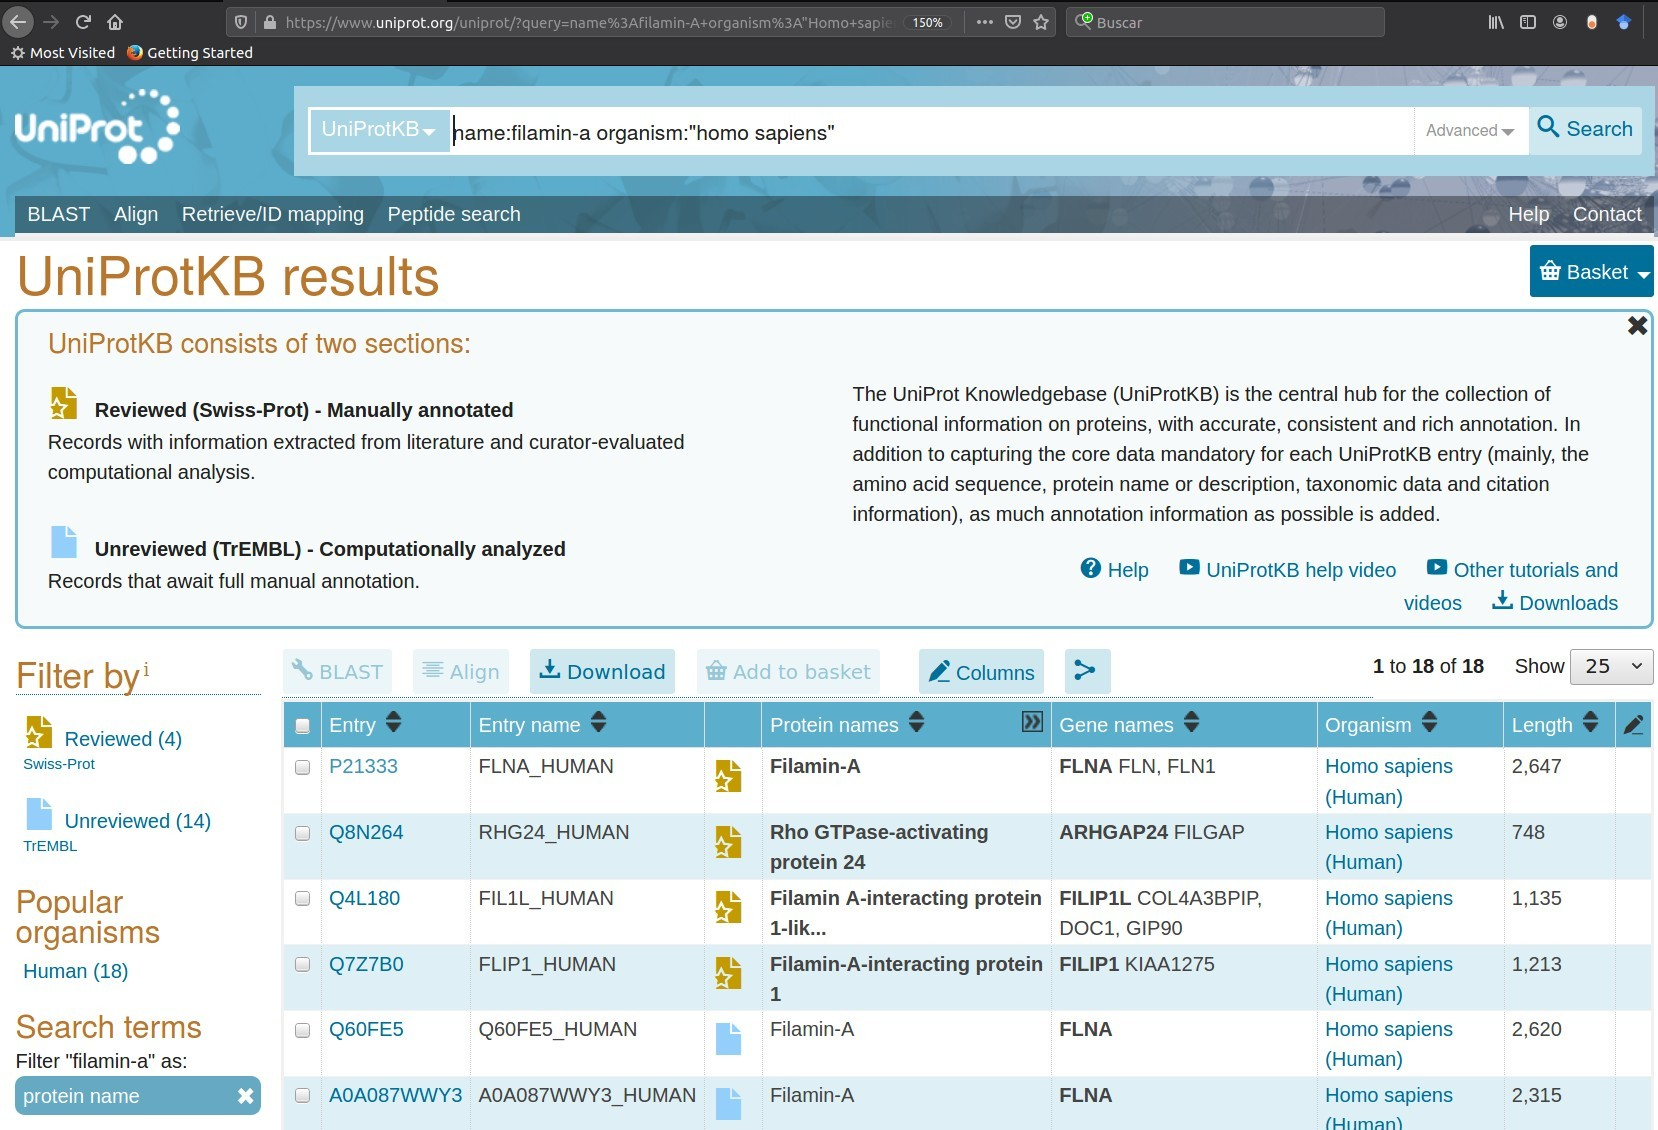
\includegraphics[width=\textwidth,height=0.6\textheight,keepaspectratio]{img/alignment/uniprot3.jpg}
    \label{img:uniprot2}
    \caption{List of results}
\end{figure}
\end{frame}
%-------------------------------------------------------
%-------------------------------------------------------

%-------------------------------------------------------
%-------------------------------------------------------
\begin{frame}{Sequence alignment}{Practice}
Look for the download button (Download isoform 1).
\begin{figure}[]
 \centering
    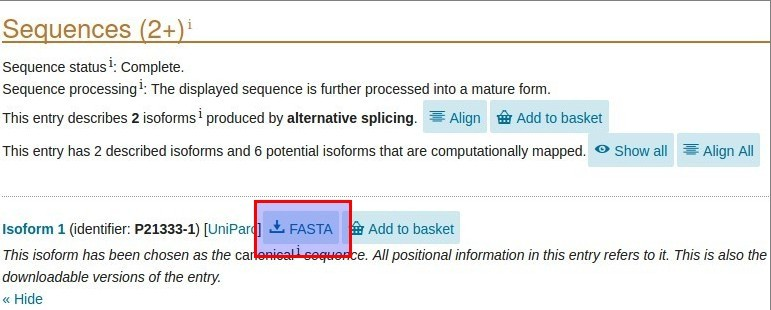
\includegraphics[width=\textwidth,height=0.6\textheight,keepaspectratio]{img/alignment/uniprot4.jpg}
    \label{img:uniprot2}
    \caption{Download the sequence}
\end{figure}
\end{frame}
%-------------------------------------------------------
%-------------------------------------------------------

%-------------------------------------------------------
%-------------------------------------------------------
\begin{frame}{Sequence alignment}{Practice}
Do the same operations for mouse species (Download the Q8BTM8 sequence, its length is \string ~2.6). 
\begin{figure}[]
 \centering
    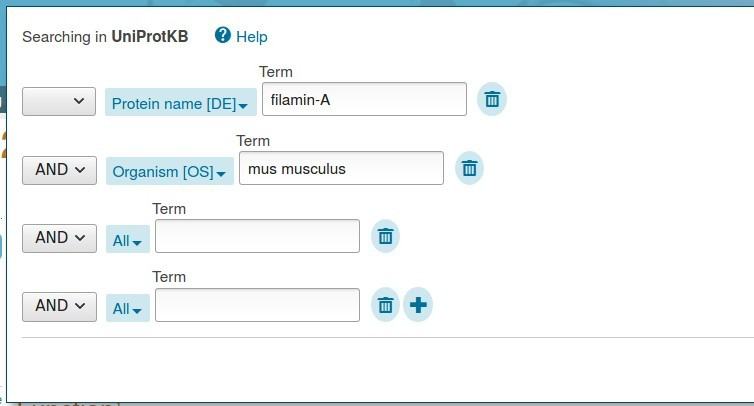
\includegraphics[width=\textwidth,height=0.6\textheight,keepaspectratio]{img/alignment/uniprot5.jpg}
    \label{img:uniprot2}
    \caption{Searching the Filamin-A protein of a mouse species}
\end{figure}
\end{frame}
%-------------------------------------------------------
%-------------------------------------------------------

%-------------------------------------------------------
%-------------------------------------------------------
\begin{frame}{Sequence alignment}{Practice}
There are several online tool to process Dot matrix: 
\begin{itemize}
    \item  \href{http://bioinfo.nhri.org.tw/cgi-bin/emboss/dotmatcher}{DotMatcher}. 
    \item  \href{https://www.ebi.ac.uk/Tools/seqstats/emboss_dotmatcher/}{EMBOSSS}.
\end{itemize}
\end{frame}
%-------------------------------------------------------
%-------------------------------------------------------


%-------------------------------------------------------
%-------------------------------------------------------
\begin{frame}{Sequence alignment}{Practice}
\begin{figure}[]
 \centering
    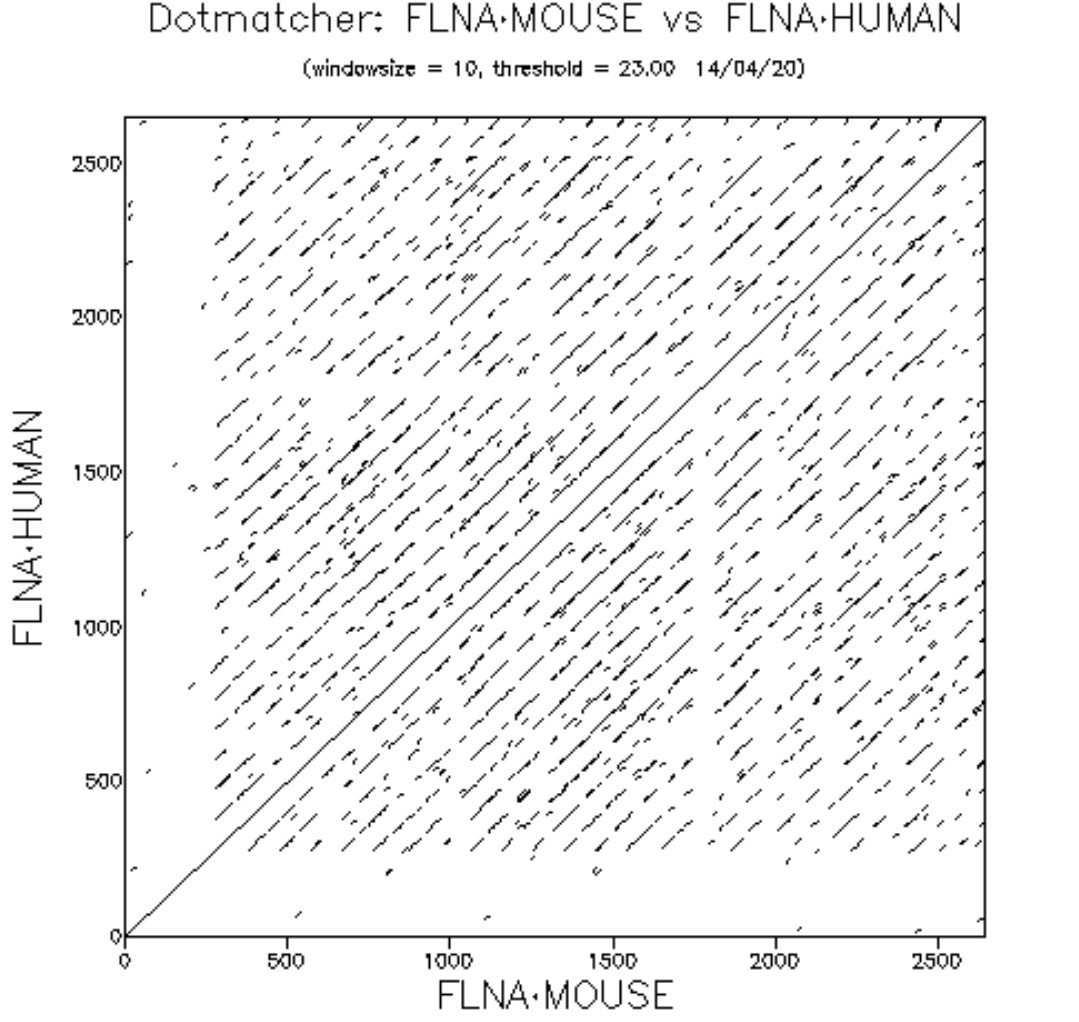
\includegraphics[width=\textwidth,height=0.6\textheight,keepaspectratio]{img/alignment/dot2.jpg}
    \label{img:uniprot2}
    \caption{Dot matrix of Filamin-A protein in human and mouse species.}
\end{figure}
\end{frame}
%-------------------------------------------------------
%-------------------------------------------------------


%-------------------------------------------------------
%-------------------------------------------------------
\begin{frame}[allowframebreaks]
        \frametitle{References}
        %\bibliographystyle{amsalpha}
        \bibliographystyle{IEEEtran}
        \bibliography{bibliography.bib}
\end{frame}
%-------------------------------------------------------
%-------------------------------------------------------

%-------------------------------------------------------
%-------------------------------------------------------
{\1
\begin{frame}[plain,noframenumbering]
  \finalpage{Thank you}
\end{frame}}
%-------------------------------------------------------
%-------------------------------------------------------



\end{document}